\documentclass[tikz]{standalone}
\usepackage{ctex}
\usepackage{tikz}
\usepackage{pgfplots}
\pgfplotsset{compat=1.18}   % 使用较新版本语法
\usetikzlibrary{positioning, arrows.meta, intersections, calc, fit, backgrounds}
\usepgfplotslibrary{fillbetween}  % 用于填充区域

\begin{document}

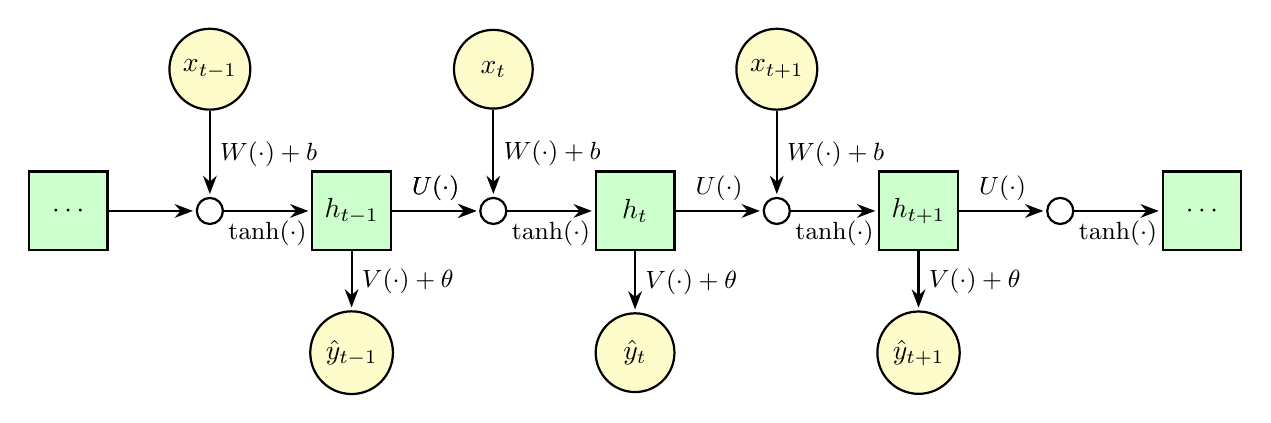
\begin{tikzpicture}[
        % ----- 全局样式 -----
        ->,>=stealth,shorten >=1pt,auto,thick,
        node distance = 1.8cm,
        >=Stealth,
        % RNN 主体 cell
        gate/.style={draw, minimum width=1cm, minimum height=1cm, fill=blue!20},
        hstate/.style={draw, minimum width=1cm, minimum height=1cm, fill=green!20},
        node/.style={circle, draw, minimum size=1cm, fill=yellow!20},
        conv/.style={circle, draw, minimum size=0.2cm}
    ]
    \node[hstate] (ht) {$h_t$};
    \node[conv, left of=ht] (convt) {};
    \node[hstate, left of=convt] (ht-1) {$h_{t-1}$};
    \node[node, above of=convt] (xt) {$x_t$};
    \node[conv, left of=ht-1] (convt-1) {};
    \node[node, above of=convt-1] (xt-1) {$x_{t-1}$};
    \node[hstate, left of=convt-1] (left) {$\cdots$};

    \node[conv, right of=ht] (convt+1) {};
    \node[hstate, right of=convt+1] (ht+1) {$h_{t+1}$};
    \node[node, above of=convt+1] (xt+1) {$x_{t+1}$};
    \node[conv, right of=ht+1] (convt+2) {};
    \node[hstate, right of=convt+2] (right) {$\cdots$};

    \node[node, below of=ht] (yt) {$\hat y_t$};
    \node[node, below of=ht-1] (yt-1) {$\hat y_{t-1}$};
    \node[node, below of=ht+1] (yt+1) {$\hat y_{t+1}$};

    % ----- 绘制箭头 -----
    \path[every node/.style={font=\sffamily\small}]
    (ht-1) edge node [above] {$U(\cdot)$} (convt)
    (convt) edge node [below] {$\tanh(\cdot)$} (ht)
    (ht) edge node [above] {$U(\cdot)$} (convt+1)
    (ht) edge node [right] {$V(\cdot)+\theta$} (yt)
    (xt) edge node [right] {$W(\cdot)+b$} (convt)
    (left) edge node [left] {} (convt-1)
    (convt-1) edge node [below] {$\tanh(\cdot)$} (ht-1)
    (ht-1) edge node [above] {$U(\cdot)$} (convt)
    (convt+1) edge node [below] {$\tanh(\cdot)$} (ht+1)
    (convt+2) edge node [below] {$\tanh(\cdot)$} (right)
    (ht+1) edge node [above] {$U(\cdot)$} (convt+2)
    (xt+1) edge node [right] {$W(\cdot)+b$} (convt+1)
    (xt-1) edge node [right] {$W(\cdot)+b$} (convt-1)
    (ht-1) edge node [right] {$V(\cdot)+\theta$} (yt-1)
    (ht+1) edge node [right] {$V(\cdot)+\theta$} (yt+1);
\end{tikzpicture}
\end{document}